\definecolor{tclblue}{HTML}{2A78D6}
\definecolor{tclorange}{HTML}{EB6834}
\definecolor{tclgray}{HTML}{8A8984}

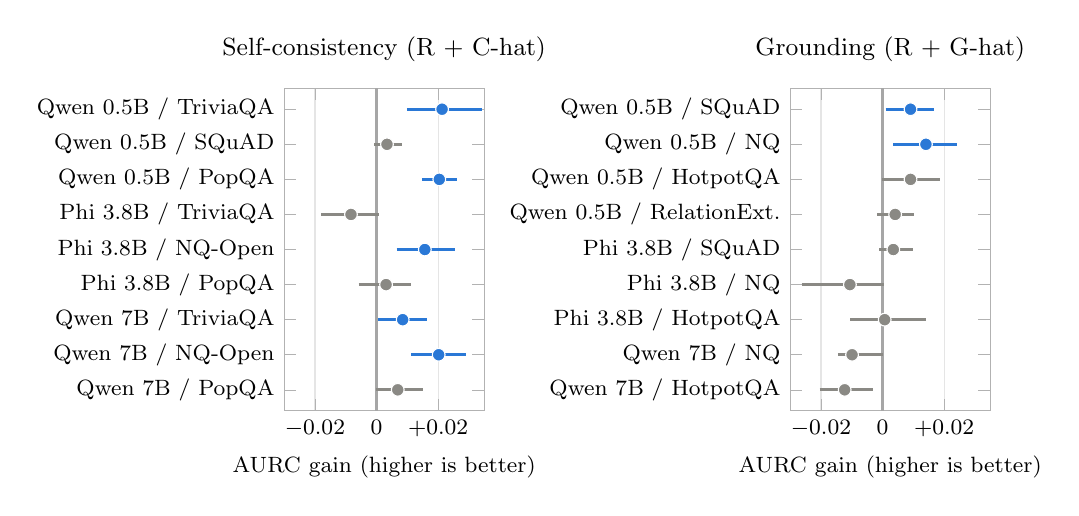
\begin{tikzpicture}
\begin{axis}[width=0.34\textwidth, height=5.68cm, xmin=-0.03, xmax=0.035, ymin=0.4, ymax=9.6, ytick={1,...,9}, yticklabels={{Qwen 0.5B / TriviaQA},{Qwen 0.5B / SQuAD},{Qwen 0.5B / PopQA},{Phi 3.8B / TriviaQA},{Phi 3.8B / NQ-Open},{Phi 3.8B / PopQA},{Qwen 7B / TriviaQA},{Qwen 7B / NQ-Open},{Qwen 7B / PopQA}}, y dir=reverse, xtick={-0.02,0,0.02}, xmajorgrids, major grid style={gray!20}, tick label style={font=\footnotesize}, label style={font=\footnotesize}, axis line style={gray!60}, tick style={gray!60}, title={Self-consistency (R + C-hat)}, title style={font=\small}, xlabel={AURC gain (higher is better)}, xticklabels={{$-$0.02},{0},{+0.02}}, scaled x ticks=false, at={(0cm,0)}]
\draw[gray!70, thick] (axis cs:0,0.4) -- (axis cs:0,9.6);
\draw[tclblue, line width=1pt] (axis cs:0.0099,1) -- (axis cs:0.0343,1);
\addplot[only marks, mark=*, mark size=2.3pt, fill=tclblue, draw=white] coordinates {(0.0213,1)};
\draw[tclgray, line width=1pt] (axis cs:-0.0008,2) -- (axis cs:0.0082,2);
\addplot[only marks, mark=*, mark size=2.3pt, fill=tclgray, draw=white] coordinates {(0.0034,2)};
\draw[tclblue, line width=1pt] (axis cs:0.0147,3) -- (axis cs:0.0263,3);
\addplot[only marks, mark=*, mark size=2.3pt, fill=tclblue, draw=white] coordinates {(0.0204,3)};
\draw[tclgray, line width=1pt] (axis cs:-0.0179,4) -- (axis cs:0.0007,4);
\addplot[only marks, mark=*, mark size=2.3pt, fill=tclgray, draw=white] coordinates {(-0.0083,4)};
\draw[tclblue, line width=1pt] (axis cs:0.0065,5) -- (axis cs:0.0255,5);
\addplot[only marks, mark=*, mark size=2.3pt, fill=tclblue, draw=white] coordinates {(0.0157,5)};
\draw[tclgray, line width=1pt] (axis cs:-0.0058,6) -- (axis cs:0.0111,6);
\addplot[only marks, mark=*, mark size=2.3pt, fill=tclgray, draw=white] coordinates {(0.0031,6)};
\draw[tclblue, line width=1pt] (axis cs:0.0006,7) -- (axis cs:0.0165,7);
\addplot[only marks, mark=*, mark size=2.3pt, fill=tclblue, draw=white] coordinates {(0.0085,7)};
\draw[tclblue, line width=1pt] (axis cs:0.0113,8) -- (axis cs:0.0291,8);
\addplot[only marks, mark=*, mark size=2.3pt, fill=tclblue, draw=white] coordinates {(0.0202,8)};
\draw[tclgray, line width=1pt] (axis cs:-0.0003,9) -- (axis cs:0.0150,9);
\addplot[only marks, mark=*, mark size=2.3pt, fill=tclgray, draw=white] coordinates {(0.0069,9)};
\end{axis}
\begin{axis}[width=0.34\textwidth, height=5.68cm, xmin=-0.03, xmax=0.035, ymin=0.4, ymax=9.6, ytick={1,...,9}, yticklabels={{Qwen 0.5B / SQuAD},{Qwen 0.5B / NQ},{Qwen 0.5B / HotpotQA},{Qwen 0.5B / RelationExt.},{Phi 3.8B / SQuAD},{Phi 3.8B / NQ},{Phi 3.8B / HotpotQA},{Qwen 7B / NQ},{Qwen 7B / HotpotQA}}, y dir=reverse, xtick={-0.02,0,0.02}, xmajorgrids, major grid style={gray!20}, tick label style={font=\footnotesize}, label style={font=\footnotesize}, axis line style={gray!60}, tick style={gray!60}, title={Grounding (R + G-hat)}, title style={font=\small}, xlabel={AURC gain (higher is better)}, xticklabels={{$-$0.02},{0},{+0.02}}, scaled x ticks=false, at={(0.53\textwidth,0)}]
\draw[gray!70, thick] (axis cs:0,0.4) -- (axis cs:0,9.6);
\draw[tclblue, line width=1pt] (axis cs:0.0010,1) -- (axis cs:0.0167,1);
\addplot[only marks, mark=*, mark size=2.3pt, fill=tclblue, draw=white] coordinates {(0.0091,1)};
\draw[tclblue, line width=1pt] (axis cs:0.0035,2) -- (axis cs:0.0242,2);
\addplot[only marks, mark=*, mark size=2.3pt, fill=tclblue, draw=white] coordinates {(0.0141,2)};
\draw[tclgray, line width=1pt] (axis cs:-0.0003,3) -- (axis cs:0.0187,3);
\addplot[only marks, mark=*, mark size=2.3pt, fill=tclgray, draw=white] coordinates {(0.0091,3)};
\draw[tclgray, line width=1pt] (axis cs:-0.0017,4) -- (axis cs:0.0103,4);
\addplot[only marks, mark=*, mark size=2.3pt, fill=tclgray, draw=white] coordinates {(0.0041,4)};
\draw[tclgray, line width=1pt] (axis cs:-0.0011,5) -- (axis cs:0.0098,5);
\addplot[only marks, mark=*, mark size=2.3pt, fill=tclgray, draw=white] coordinates {(0.0035,5)};
\draw[tclgray, line width=1pt] (axis cs:-0.0263,6) -- (axis cs:0.0004,6);
\addplot[only marks, mark=*, mark size=2.3pt, fill=tclgray, draw=white] coordinates {(-0.0106,6)};
\draw[tclgray, line width=1pt] (axis cs:-0.0105,7) -- (axis cs:0.0140,7);
\addplot[only marks, mark=*, mark size=2.3pt, fill=tclgray, draw=white] coordinates {(0.0007,7)};
\draw[tclgray, line width=1pt] (axis cs:-0.0145,8) -- (axis cs:0.0001,8);
\addplot[only marks, mark=*, mark size=2.3pt, fill=tclgray, draw=white] coordinates {(-0.0099,8)};
\draw[tclgray, line width=1pt] (axis cs:-0.0204,9) -- (axis cs:-0.0032,9);
\addplot[only marks, mark=*, mark size=2.3pt, fill=tclgray, draw=white] coordinates {(-0.0123,9)};
\end{axis}
\end{tikzpicture}
